\section{Appendix}
Tutorial exercises.

\begin{equation}
\int_0^\pi \sin(x) \, dx
\label{eq:}
\end{equation}

\begin{figure}[h]
	\centering
		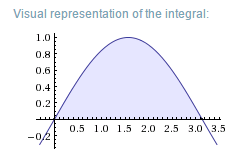
\includegraphics{graphics/intsinx.png}
	\caption{$sin(x)$}
	\label{fig:intsinx}
\end{figure}


\subsection{Integration with the 'simple rules'}
\begin{enumerate}
	\item Estimate the exact solution to the integral
	\item Use the Midpoint, Trapezoid and Simpson's rule to approximate the integral.
	\item Use the composite trapezoid rule for two and four intervals to approximate the integral.
\end{enumerate}


\subsubsection{Solution}
$a = 0, b = \pi$

\begin{enumerate}
	\item Solving the integral:
	\begin{equation}
\int_0^\pi \sin(x) \, dx = -\cos(x) \Big|_{x=0}^{x=\pi} = 2
\label{sol:int}
\end{equation}
	
	\item Solution for midpoint (\ref{sol:midpoint}), trapezoid (\ref{sol:trapezoid_rule}) and simpson's (\ref{sol:simpsons}) rule to approximate the integral.	
	
	\begin{equation}
\int\limits_{a}^{b} f(x)\, dx \approx (b - a) \cdot f\!\left(\frac{a + b}{2}\right) 
= (\pi) \cdot \sin{\!\left(\frac{\pi}{2}\right)} = \pi
 \label{sol:midpoint}
\end{equation}
	
	\begin{equation}
 \int_{a}^{b} f(x)\, dx \approx (b-a) \left[\frac{f(a) + f(b)}{2} \right] = \pi * \frac{0}{2} = 0
 \label{sol:trapezoid_rule}
\end{equation}
	
	
	\begin{equation}
 \int_{a}^{b} f(x) \, dx \approx \tfrac{b-a}{6}\left[f(a) + 4f\left(\tfrac{a+b}{2}\right)+f(b)\right]
 = \tfrac{\pi}{6}\left[4 \sin \left(\tfrac{\pi}{2}\right)\right] =  \frac{2 \pi}{3} \approx 2.094
\label{sol:simpsons}
\end{equation}
	
	
	\item Application of the composite trapezoid rule on two intervals:
	
	$a_1 = 0, b_1 = a_2 = \pi / 2, b_2 = \pi$
	
	\begin{equation}
 \int_{0}^{\frac{\pi}{2}} \sin(x)\, dx \approx \frac{\pi}{2} \left[\frac{\sin(0) + \sin(\frac{\pi}{2})}{2} \right] = \frac{\pi}{4}
 \label{sol:trleft}
\end{equation}

\begin{equation}
 \int_{\frac{\pi}{2}}^{\pi} \sin(x)\, dx \approx \frac{\pi}{2} \left[\frac{\sin(\frac{\pi}{2}) + \sin(\pi)}{2} \right] = \frac{\pi}{4}
 \label{sol:trright}
\end{equation}

\begin{equation}
 \int_{0}^{\frac{\pi}{2}} \sin(x)\, dx + \int_{\frac{\pi}{2}}^{\pi} \sin(x)\, dx \approx \frac{\pi}{2} = 1.571
 \label{sol:add}
\end{equation}

\begin{figure}
	\centering
		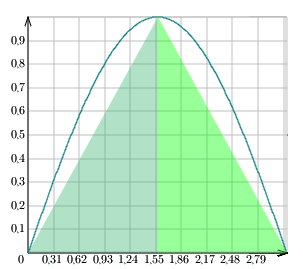
\includegraphics[width=0.50\textwidth]{graphics/trapezn2.png}
	\caption{Trapezoid rule for n = 2}
	\label{fig:trapezn2}
\end{figure}


	
	\item Application of the composite trapezoid rule on four intervals:
	
	\begin{equation}
 \int_0^\pi \sin(x) \, dx = 
 \int_{0}^{\frac{\pi}{4}} \sin(x)\, dx 
+\int_{\frac{\pi}{4}}^{\frac{\pi}{2}} \sin(x)\, dx 
+ \int_{\frac{\pi}{2}}^{\frac{3\pi}{4}} \sin(x)\, dx 
+\int_{\frac{3\pi}{4}}^{\frac{\pi}{2}} \sin(x)\, dx 
= \dots \approx 1.8961
\end{equation}
	
\begin{figure}
	\centering
		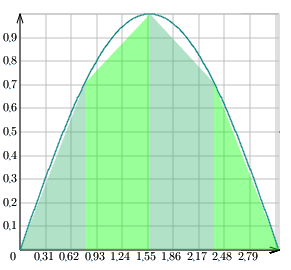
\includegraphics[width=0.50\textwidth]{graphics/trapezn4.png}
	\caption{Trapezoid rule for n=4}
	\label{fig:trapezn4}
\end{figure}	
	
\end{enumerate}


\subsection{Gaussian Quadrature}
Transform the interval from $[0, \pi]$ to $[-1, 1]$ and apply the Gaussian quadrature rule for $n=2$

\subsubsection{Interval Transformation}

The formula from section \ref{sec:gauss_quad}

\begin{equation}
\int_a^b f(x)\,dx = \frac{b-a}{2} \int_{-1}^1 f\left(\frac{b-a}{2}x + \frac{a+b}{2}\right)\,dx
\end{equation}

Applied to our integral

\begin{equation}
\int_0^\pi \sin(x) \, dx = \frac{\pi}{2} \int_{-1}^1 \sin\left(\frac{\pi}{2}x + \frac{\pi}{2}\right)\,dx
\end{equation}

\subsubsection{Application of the Gaussian Quadrature Rule}

The tranforme interval

\begin{equation}
\frac{\pi}{2} \int_{-1}^1 \sin\left(\frac{\pi}{2}x + \frac{\pi}{2}\right)\,dx
\end{equation}

The Gaussian two-point rule:
$$\int_{-1}^1 f(x) \, dx \approx f(- \frac{1}{\sqrt{3}} ) + f( \frac{1}{\sqrt{3}} )$$

Deployed:

\begin{equation}
\frac{\pi}{2} \int_{-1}^1 \sin\left(\frac{\pi}{2}x + \frac{\pi}{2}\right)\,dx
= \frac{\pi}{2} \left( \int_{-1}^1 f'(x) \, dx \right)
\approx  \frac{\pi}{2} \left( f'(- \frac{1}{\sqrt{3}} ) + f'( \frac{1}{\sqrt{3}} ) \right)
\end{equation}

\begin{equation}
f'(x) = \sin\left(\frac{\pi}{2}x + \frac{\pi}{2}\right)
\end{equation}

\begin{equation}
f'(\pm \frac{1}{\sqrt{3}}) = 0.6162
\end{equation}

\begin{equation}
=> \frac{\pi}{2} \int_{-1}^1 \sin\left(\frac{\pi}{2}x + \frac{\pi}{2}\right)\,dx
\approx \frac{\pi}{2} * 0.6162 = 1,936
\end{equation}


\newpage

\subsection{Comparison}
Compare the results.

\subsubsection{Solution}
\begin{itemize}
	\item [Exact: ] 2
	\item [Midpoint: ] $\pi$
	\item [Trapezoid n = 1:] 0
	\item [Trapezoid n = 2: ] $1.571$
	\item [Trapezoid n = 4:] $1.896$
	\item [Simpson's: ] $2.094$
	\item [Gaussian n = 1: ] $1.936$
\end{itemize}

The trapezoid rule for n = 1 has the worst result. However, one can see how the results get better when the interval is subdivided and more points are considered. This fact is also clearly visible when viewing the corresponding figures. The Simpson's rule is close but the Gaussian rule provides the best result while only using two points. The midpoint rule uses only one point and thus provides also a bad approximation but one can image that its performance increases when the interval is subdivided as with the trapezoid rule.




